\documentclass{beamer}

\mode<presentation>{\usetheme{Madrid}}
\usepackage{graphicx}
\usepackage{multimedia}
\usepackage{hyperref}

\usepackage[utf8]{inputenc}
\usepackage[ngerman]{babel}
\usepackage{amsmath, amssymb, amsthm}

\usepackage{subcaption}
\usepackage[T1]{fontenc}
%\usepackage[sort&compress]{natbib}

\usepackage{lmodern}
\usepackage{caption}


\author[Jan Niclas Ruppenthal, Michael Feldmann, Philipp Geier]{}
\title[]{1. Übung zur Vorlesung
Virtual Reality\\ Ames-Raum}
\institute[Universität Trier]{}
\date[06. Mai 2024]{}
\beamertemplatenavigationsymbolsempty
\setbeamertemplate{footline}
{
  \leavevmode%
  \hbox{%
  \begin{beamercolorbox}[wd=.50\paperwidth,ht=2.25ex,dp=1ex,center]{author in head/foot}%
    \usebeamerfont{author in head/foot}\insertshortauthor%~~\beamer@ifempty{\insertshortinstitute}{}{(\insertshortinstitute)}
  \end{beamercolorbox}%
  \begin{beamercolorbox}[wd=.50\paperwidth,ht=2.25ex,dp=1ex,right]{date in head/foot}%
    \usebeamerfont{date in head/foot}\insertshortdate{}\hspace*{2em}
    \insertframenumber{} / \inserttotalframenumber\hspace*{2ex} 
  \end{beamercolorbox}}%
  \vskip0pt%
}
%—-------------------------------------------------------------

\begin{document}
{
  \usebackgroundtemplate{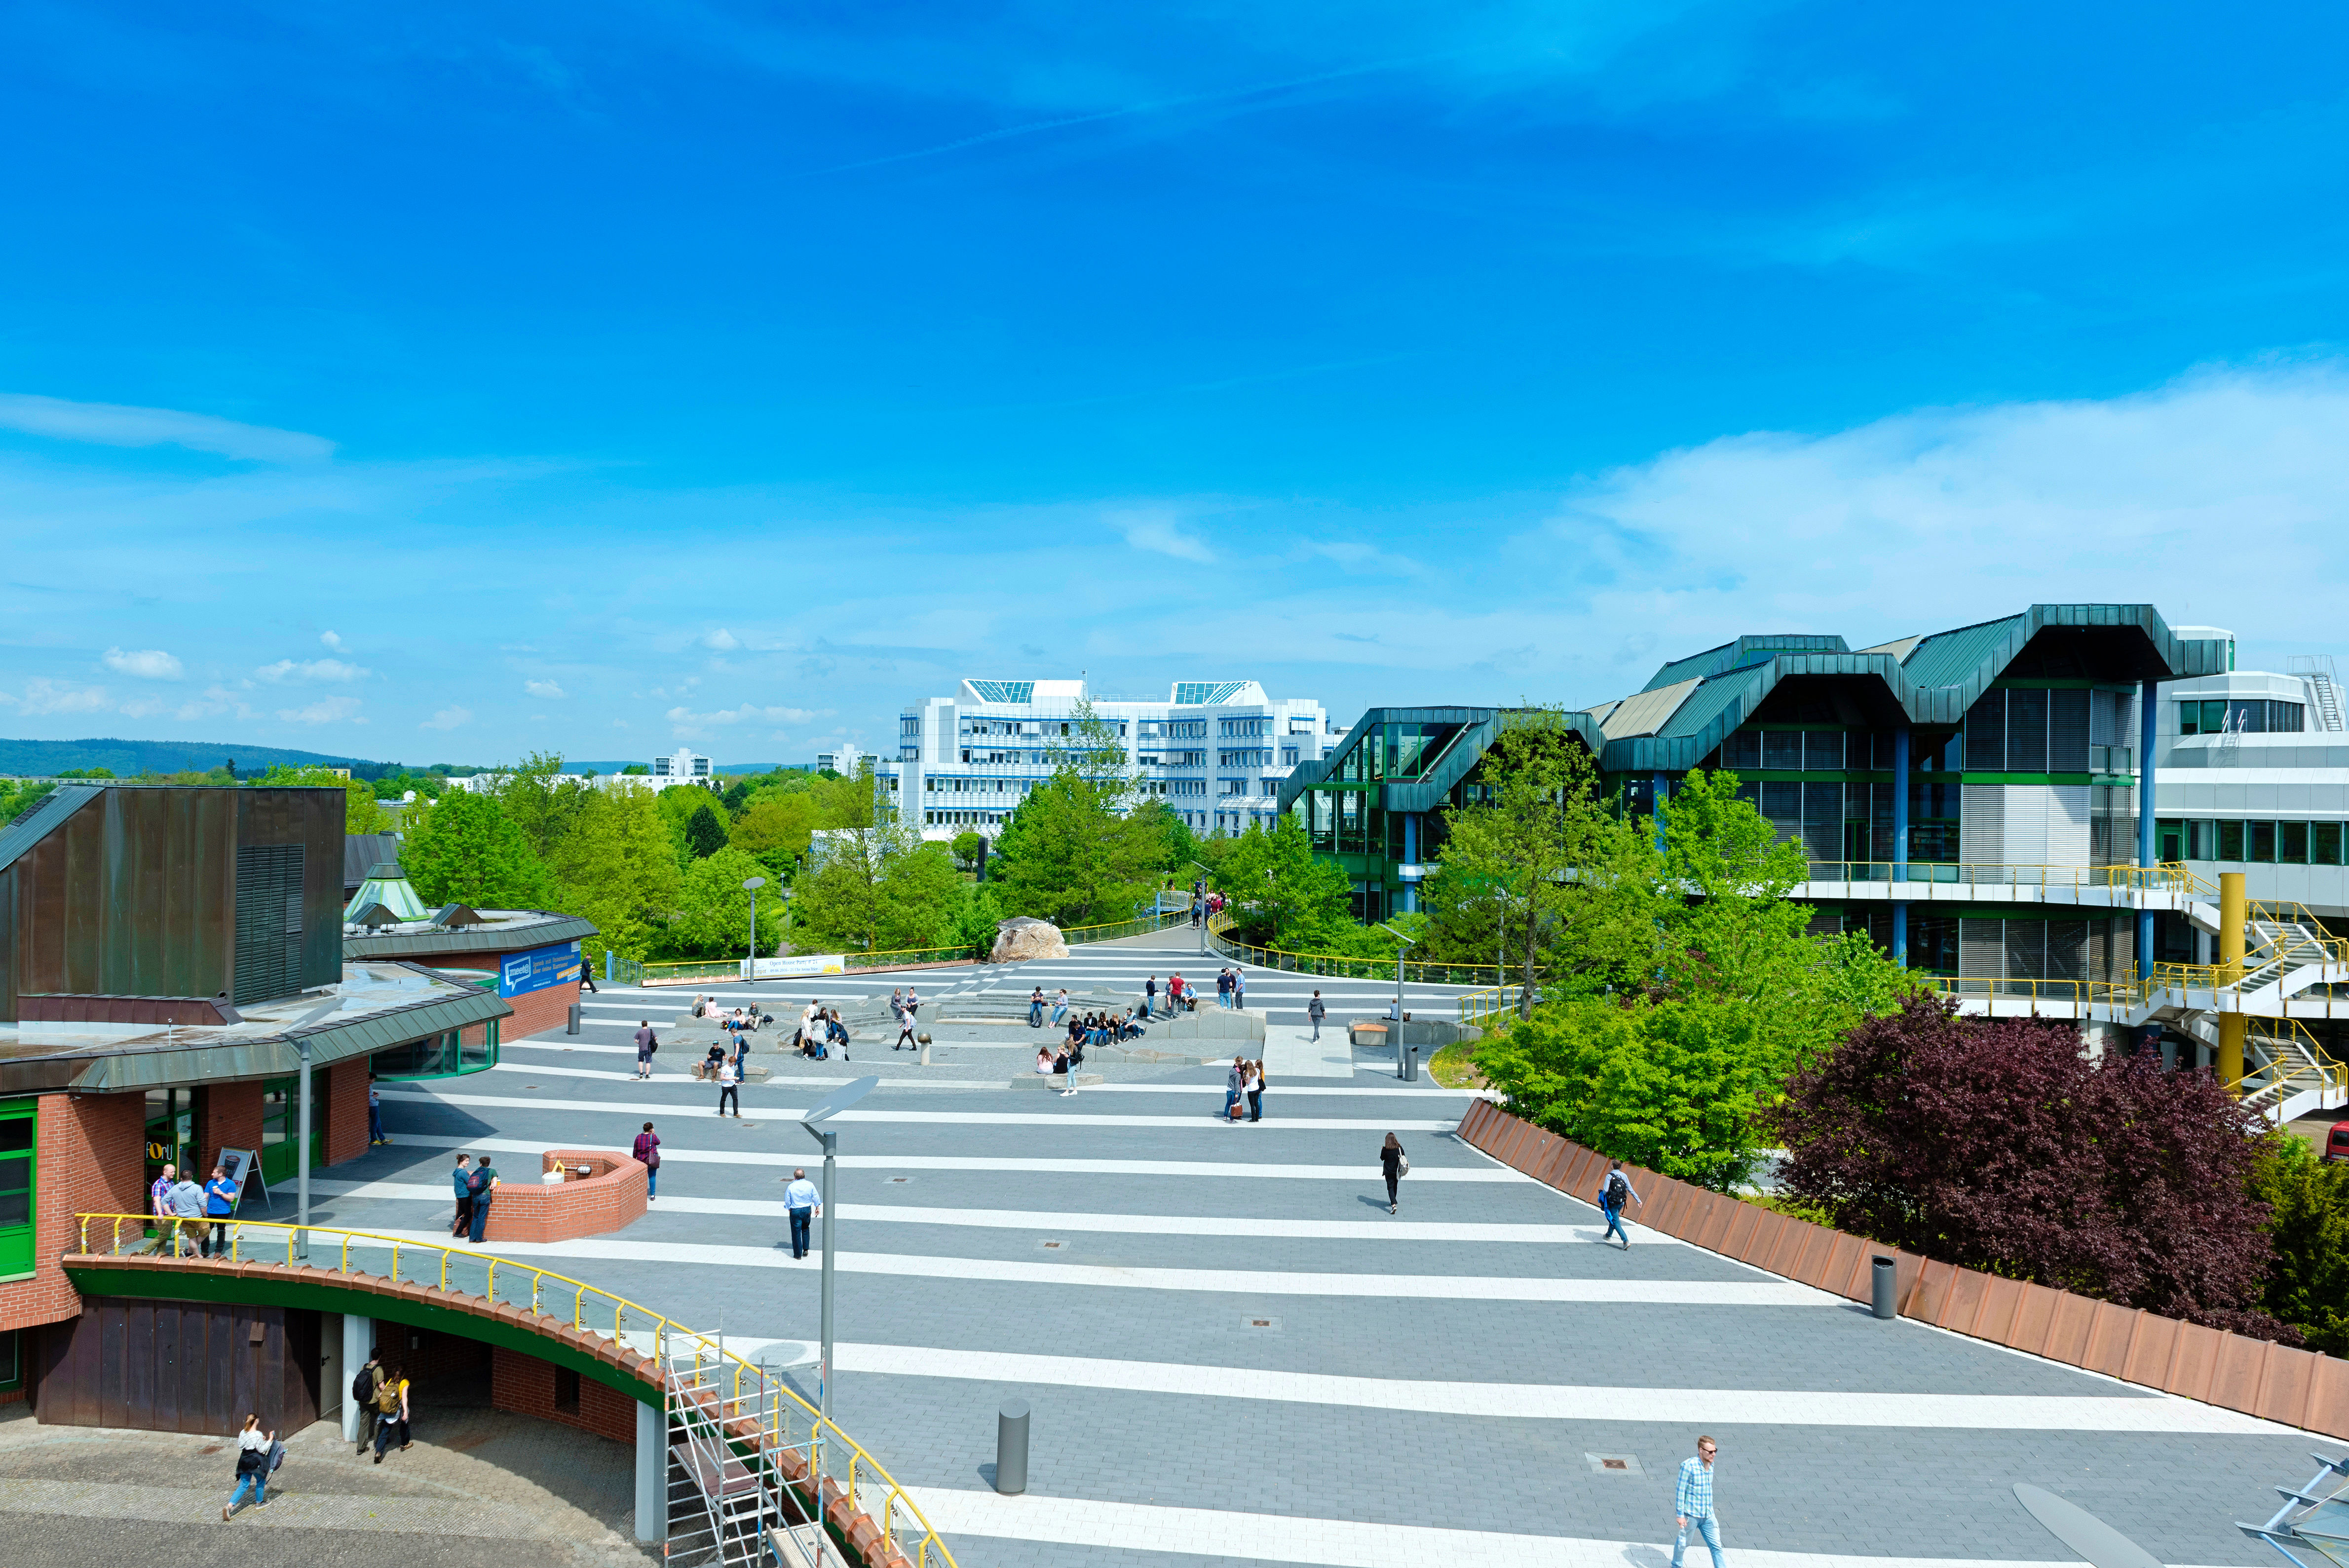
\includegraphics[width=1.2\paperwidth]{unitrier}}
  \begin{frame}
    \maketitle
  \end{frame}
}
    
    %\begin{frame}
       % \frametitle{Inhalt}
		%\tableofcontents
	%\end{frame}
	
%—------------------------------------------------------


\begin{frame}{Aufgabenteil (a)}
\begin{itemize}
\item Erstellen eines Ames-Raums in Unity
\item Verstärkung der Illusion durch die Bewegung der Charaktere
\item Auflösung der Illusion durch eine Kamerafahrt
\end{itemize}
\end{frame}

\begin{frame}{Kamerafahrt (Version 1)}
\begin{figure}
    \centering
    \movie[externalviewer]{
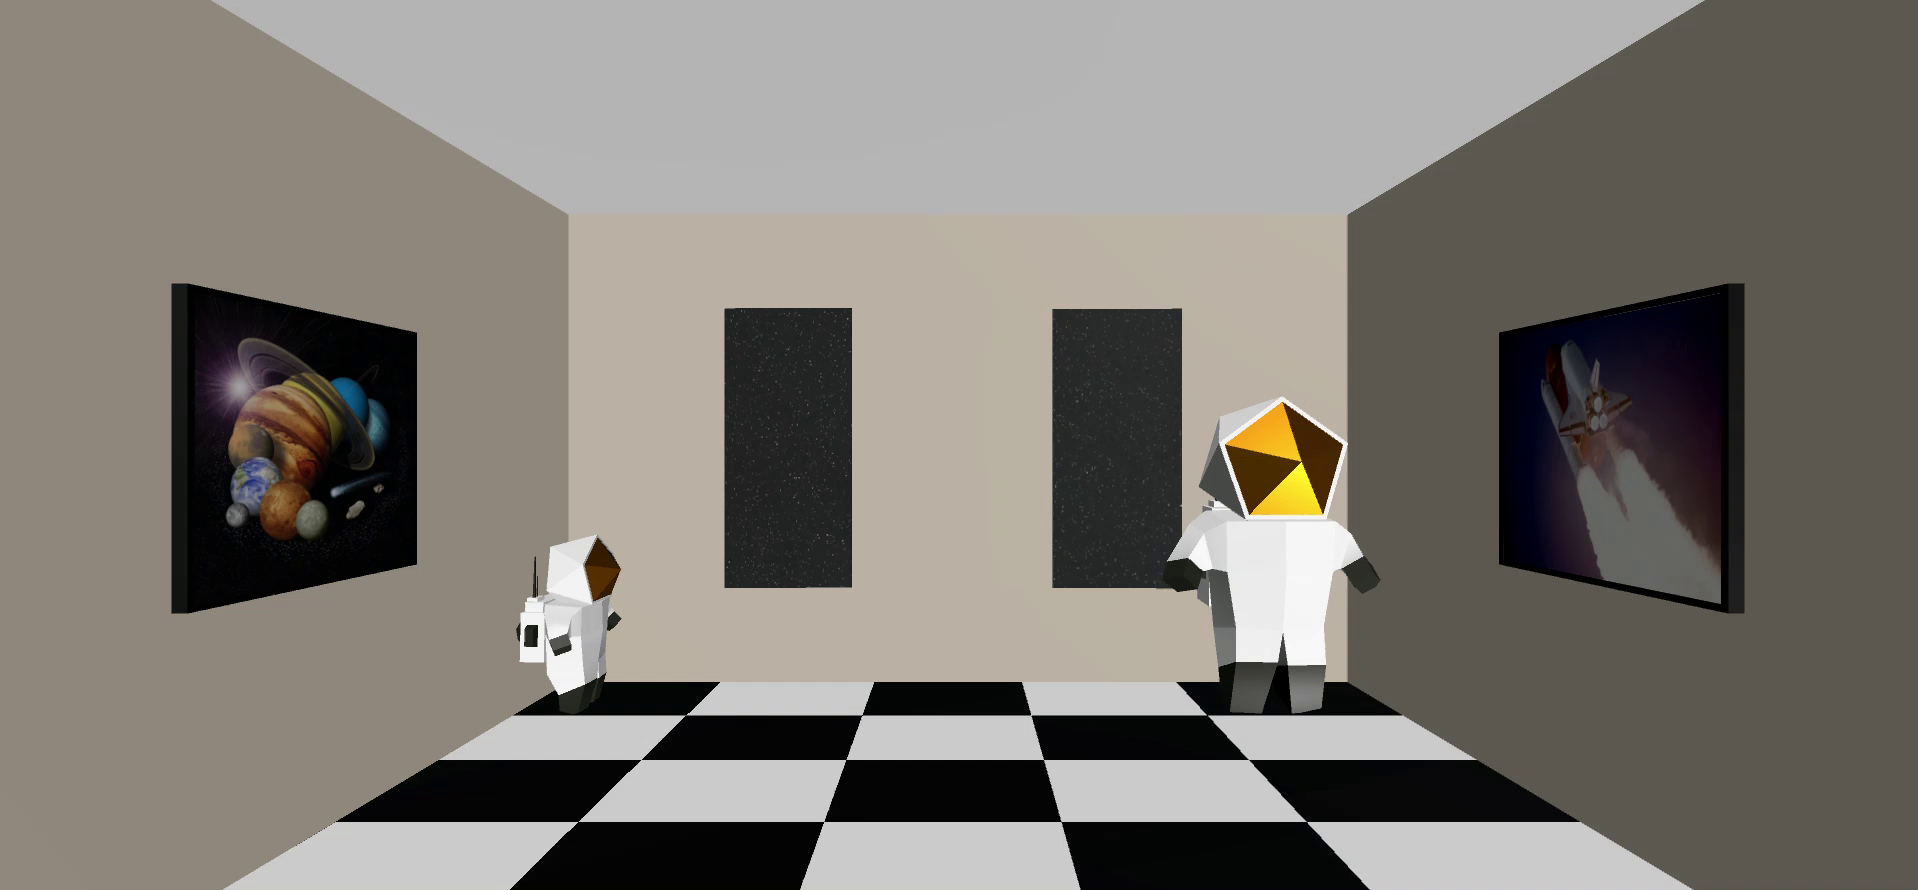
\includegraphics[width=0.9\textwidth, keepaspectratio]{NoWall-Frame}
}{MovementAmesRoom.mp4}
\caption{Kamerafahrt im Unity Editor ohne Wand}
\end{figure}
\end{frame}

\begin{frame}{Kamerafahrt (Version 2)}
\begin{figure}
    \centering
    \movie[externalviewer]{
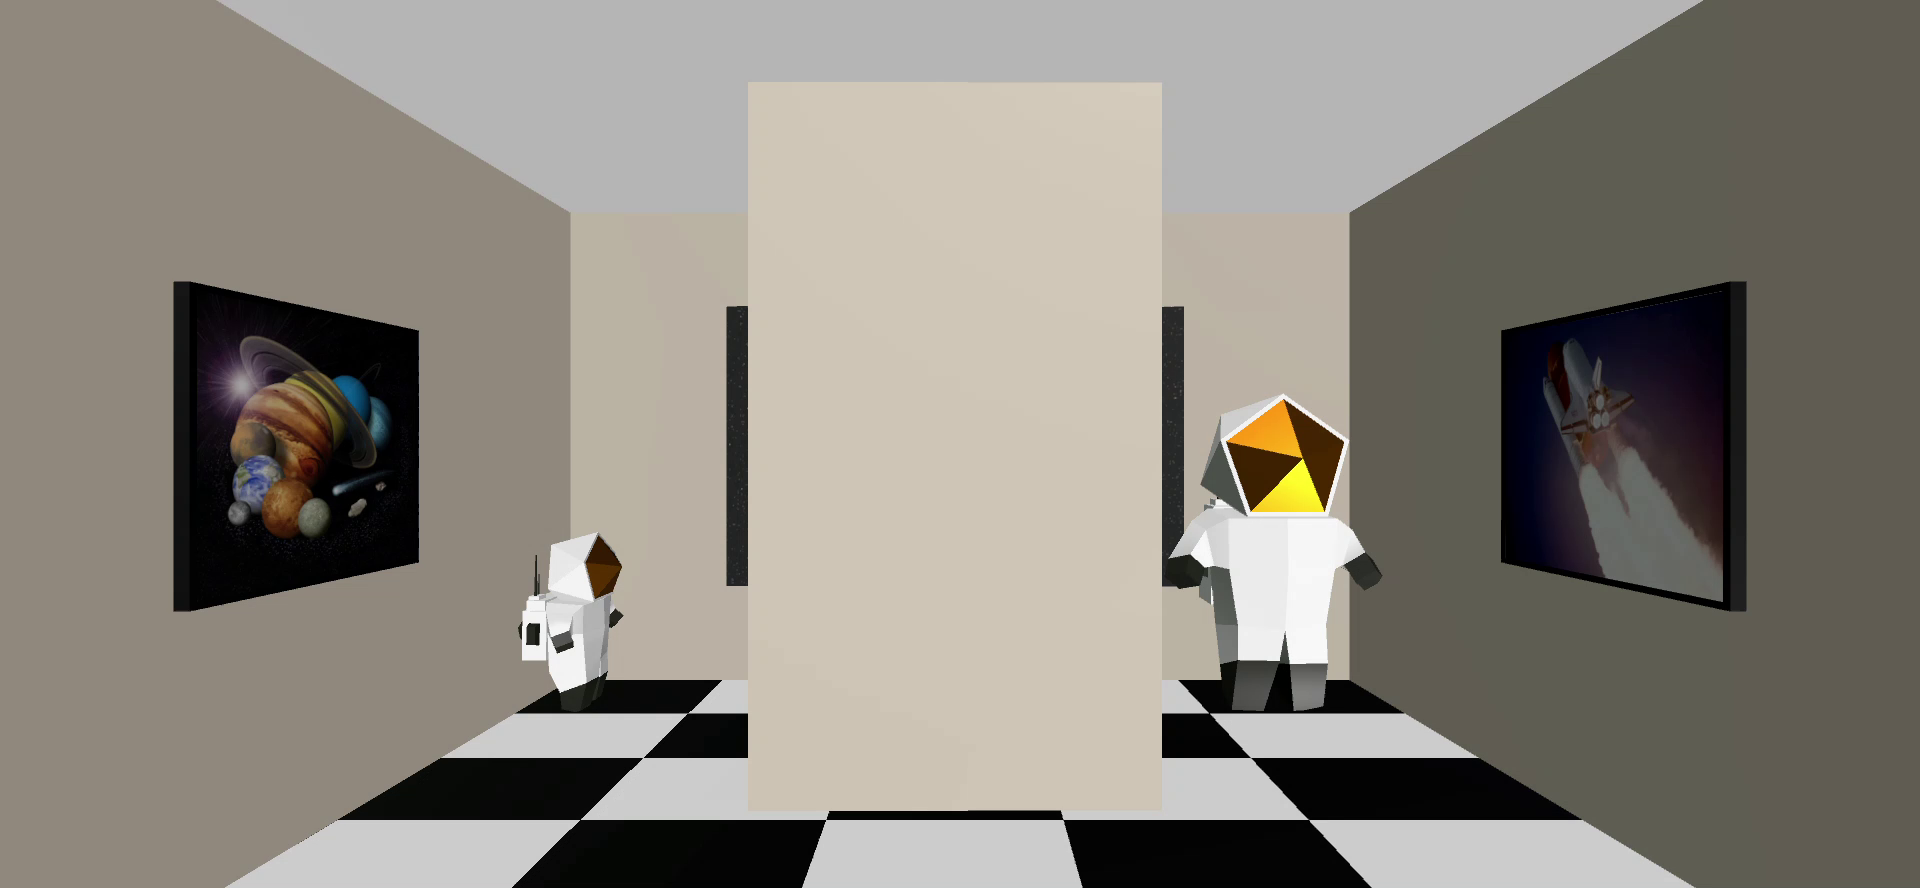
\includegraphics[width=0.9\textwidth, keepaspectratio]{Wall-Frame}
}{MovementAmesRoomWall.mp4}
\caption{Kamerafahrt im Unity Editor mit Wand}
\end{figure}
\end{frame}


\begin{frame}{Aufbau der vorderen Wand}
\begin{figure}
    \centering
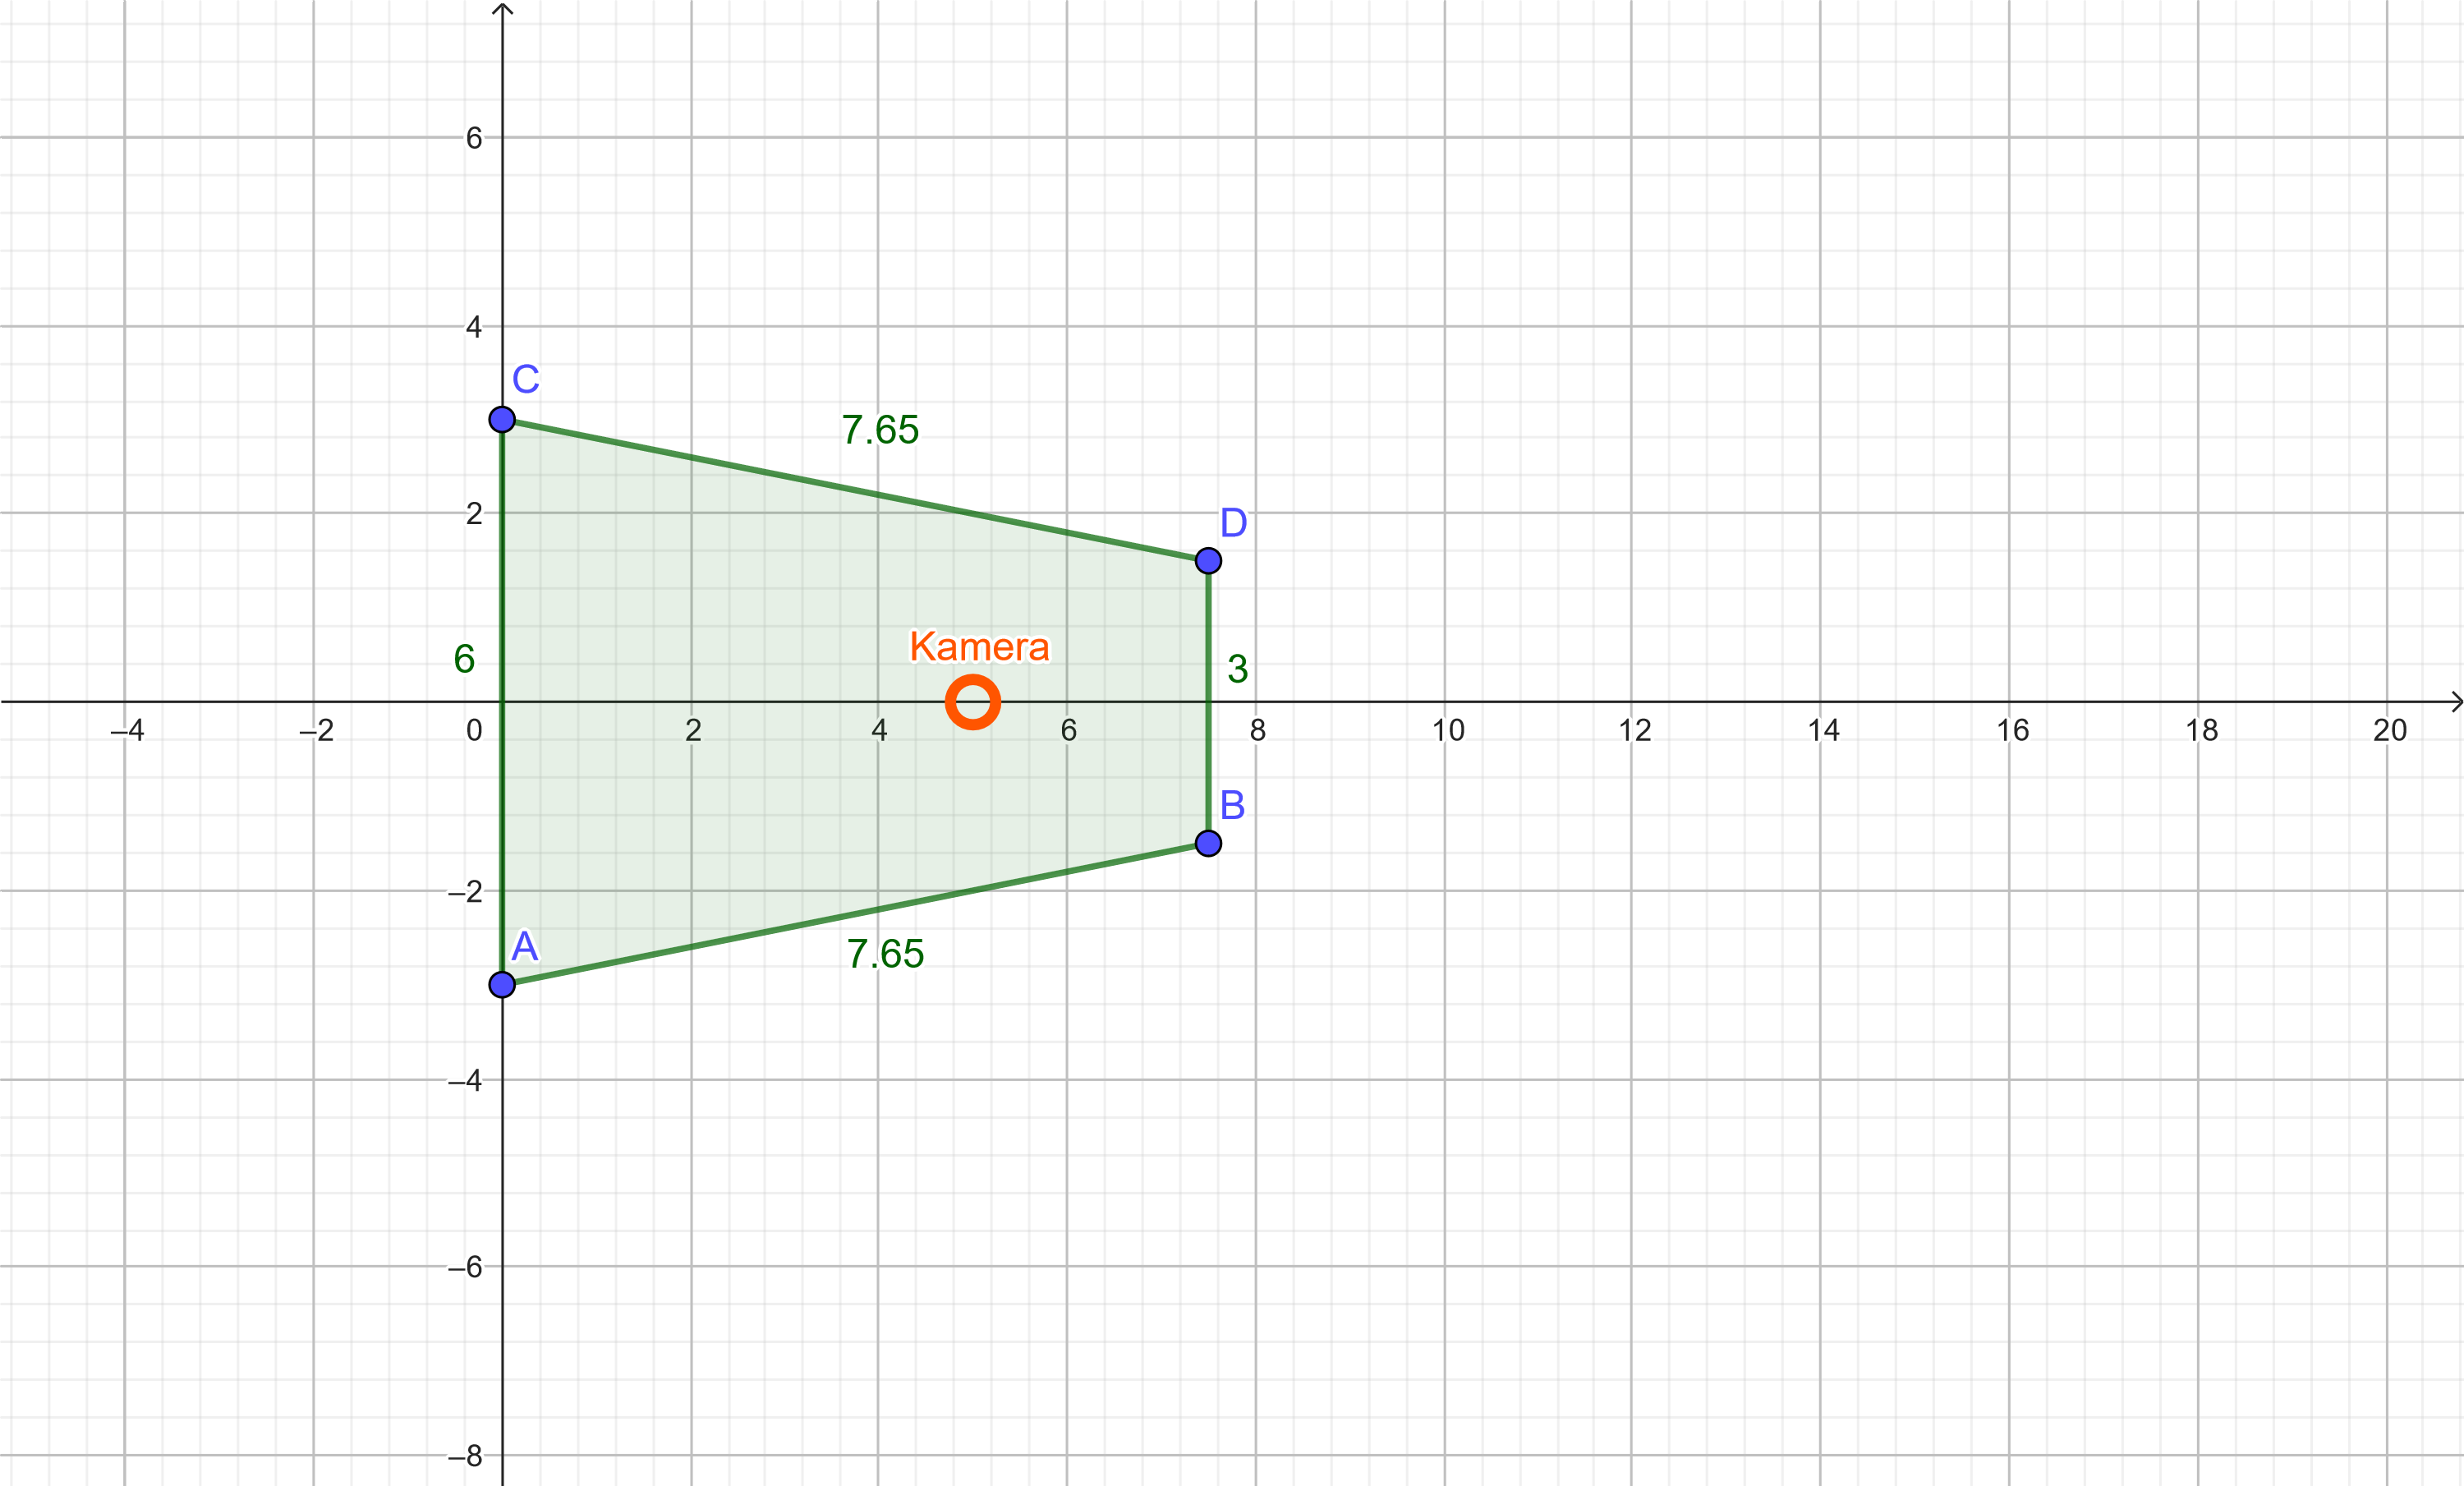
\includegraphics[width=0.9\textwidth, keepaspectratio]{geogebra-export_Vorderseite}
\caption{Maße der vorderen Wand}
\end{figure}
\end{frame}


\begin{frame}{Aufbau des Bodens}
\begin{figure}
    \centering
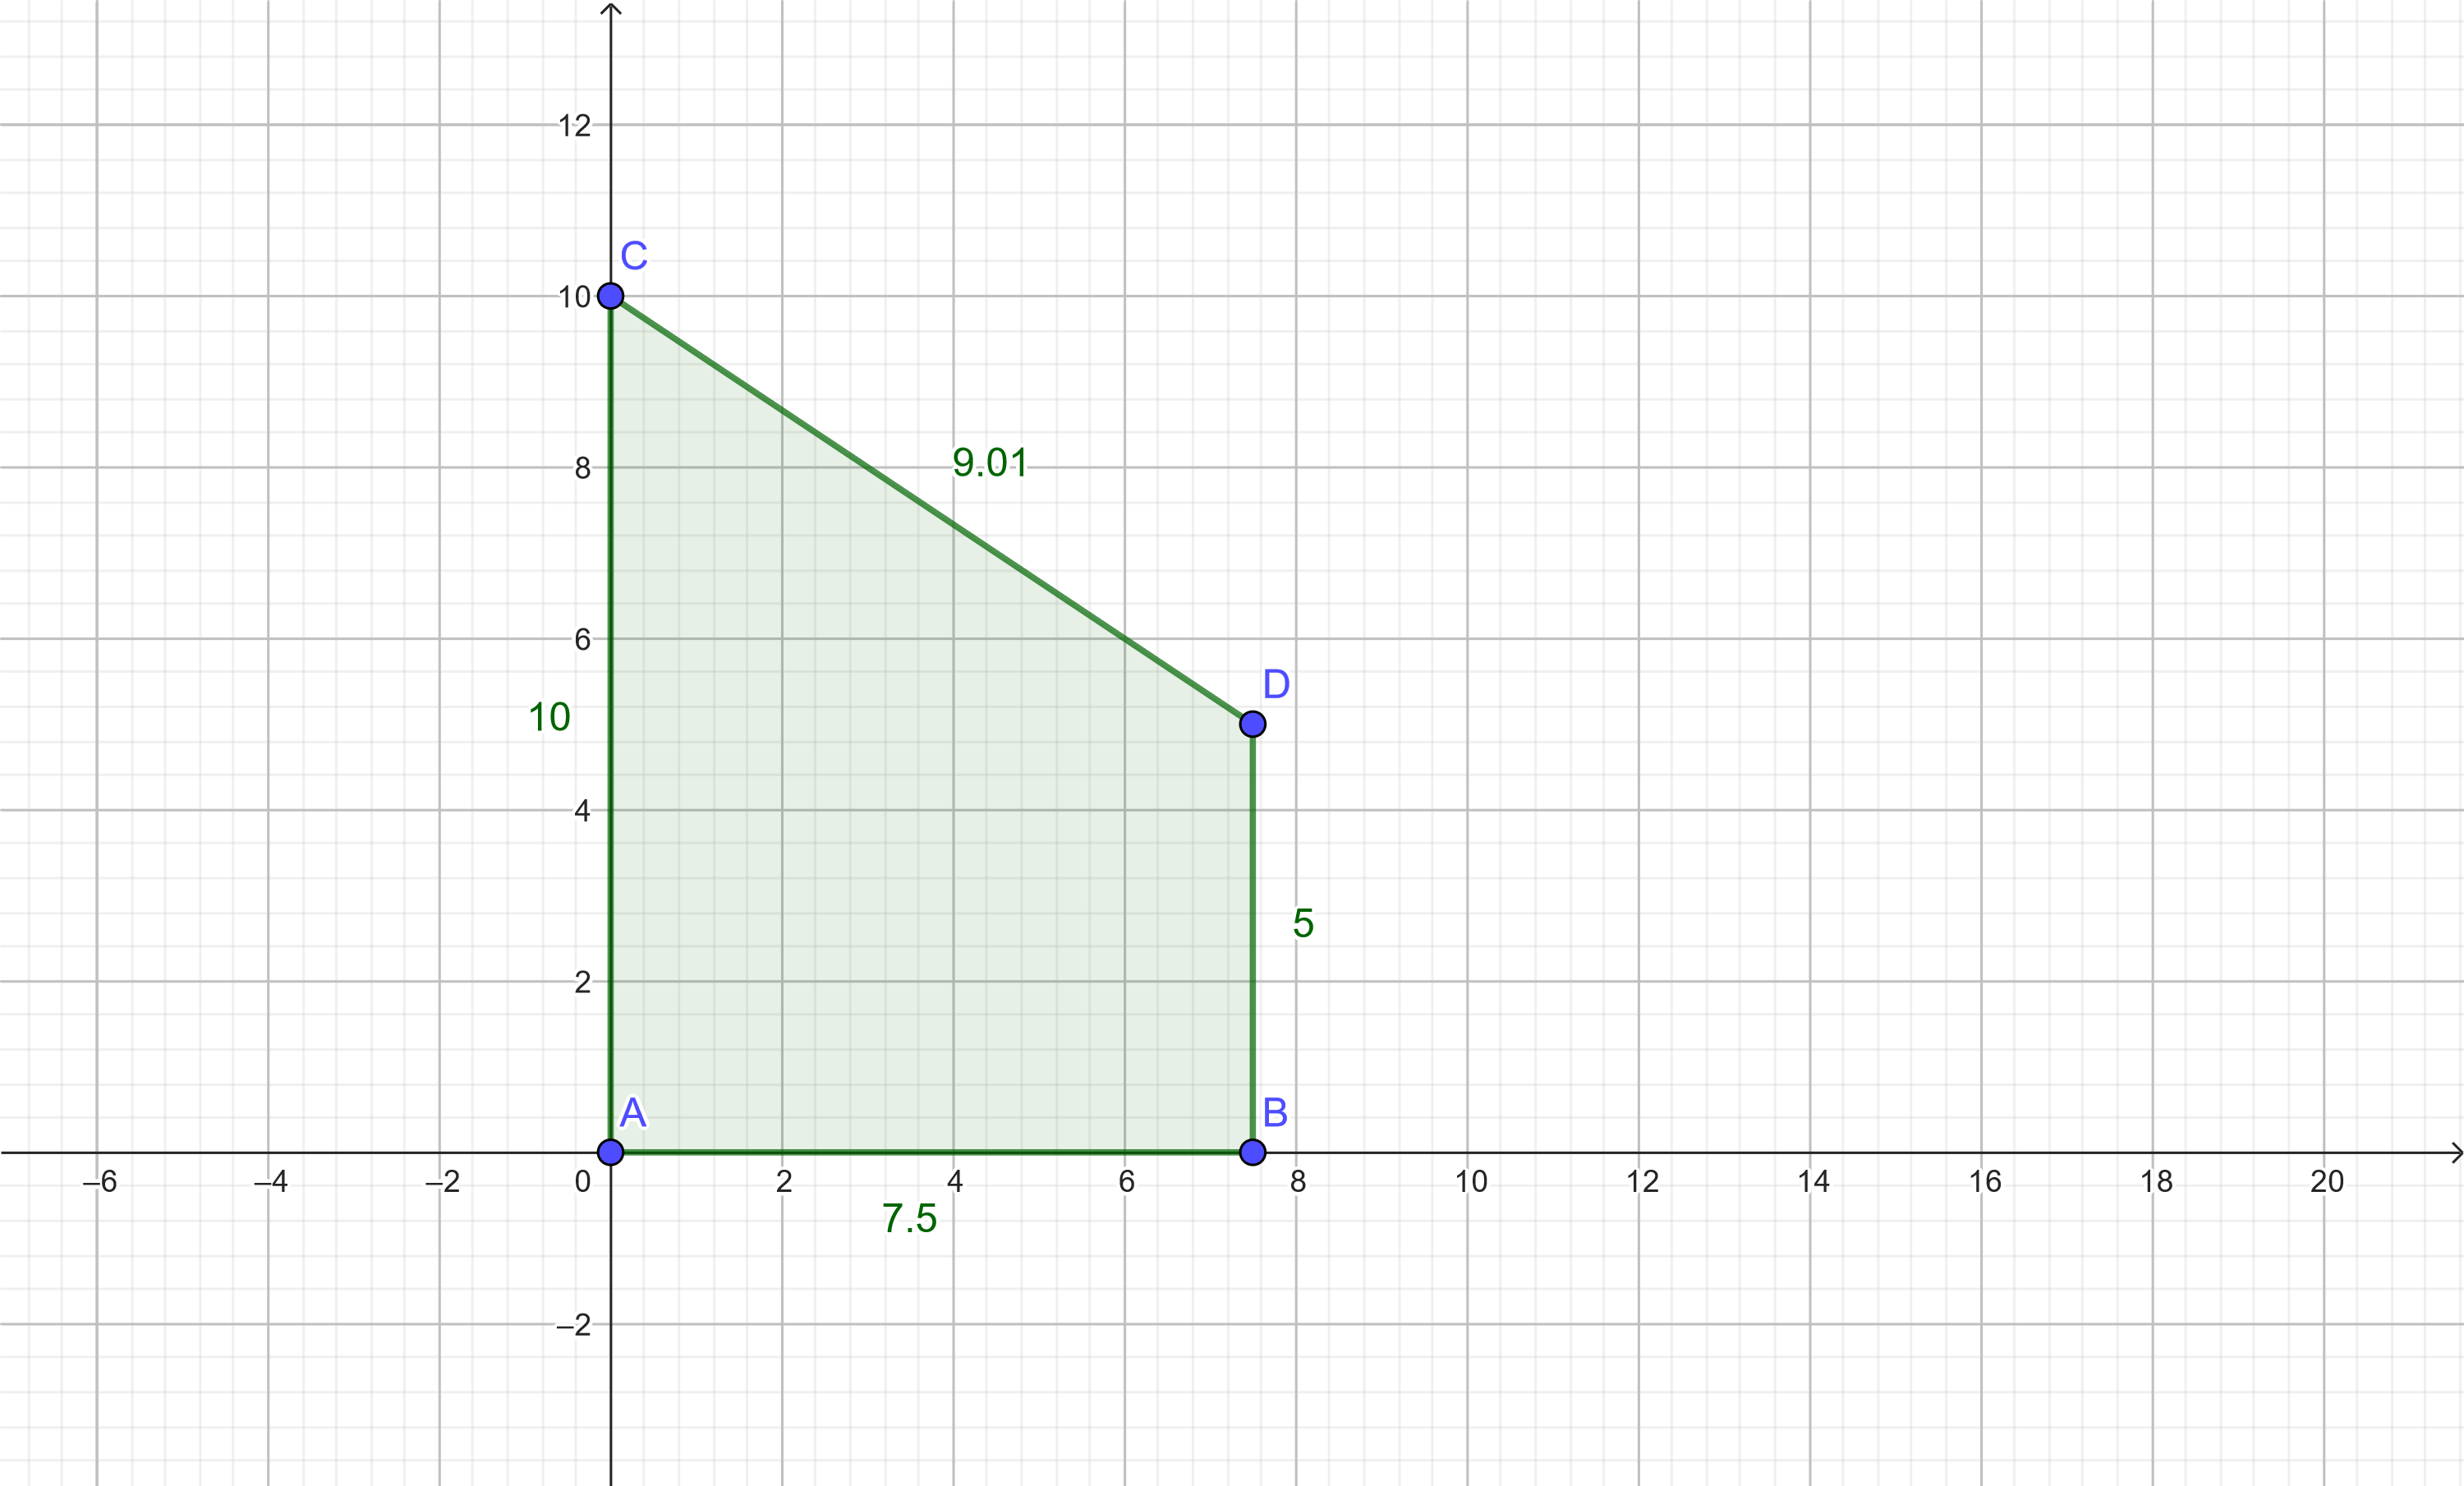
\includegraphics[width=0.9\textwidth, keepaspectratio]{geogebra-export_Boden}
\caption{Maße des Bodens}
\end{figure}
\end{frame}



\begin{frame}{Hinzufügen der Bodentextur}
\begin{figure}
    \centering
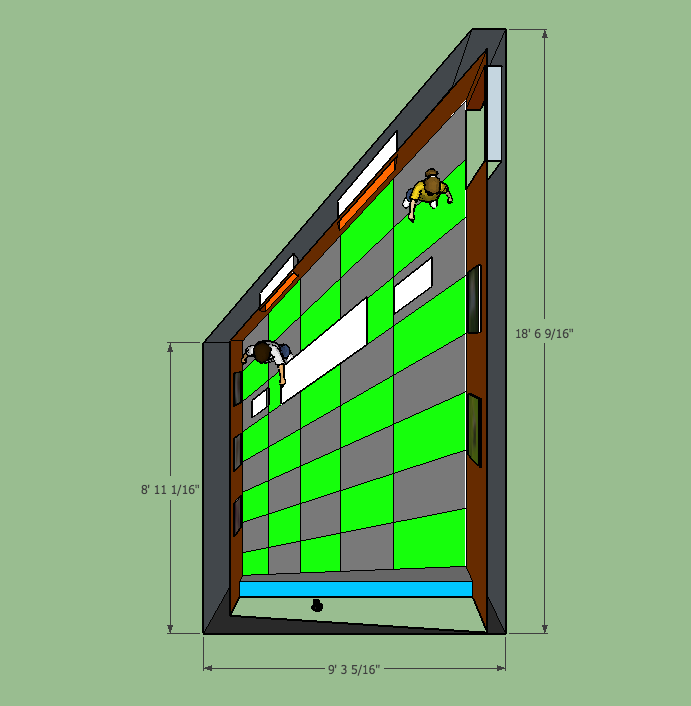
\includegraphics[width=0.75\textheight, keepaspectratio]{nick}
\caption{Checkerboard Boden \cite{nick}}
\end{figure}
\end{frame}



\begin{frame}{Prototyp}
\begin{figure}
    \centering
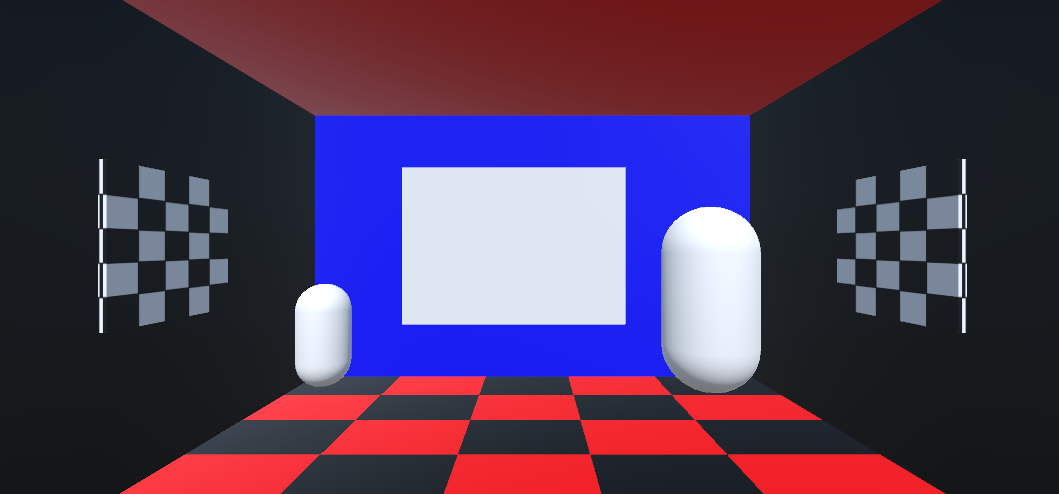
\includegraphics[width=0.9\textwidth, keepaspectratio]{prototyp}
\caption{Ames-Raum Prototyp}
\end{figure}
\end{frame}


\begin{frame}{Thematisierung}
\begin{figure}
    \centering
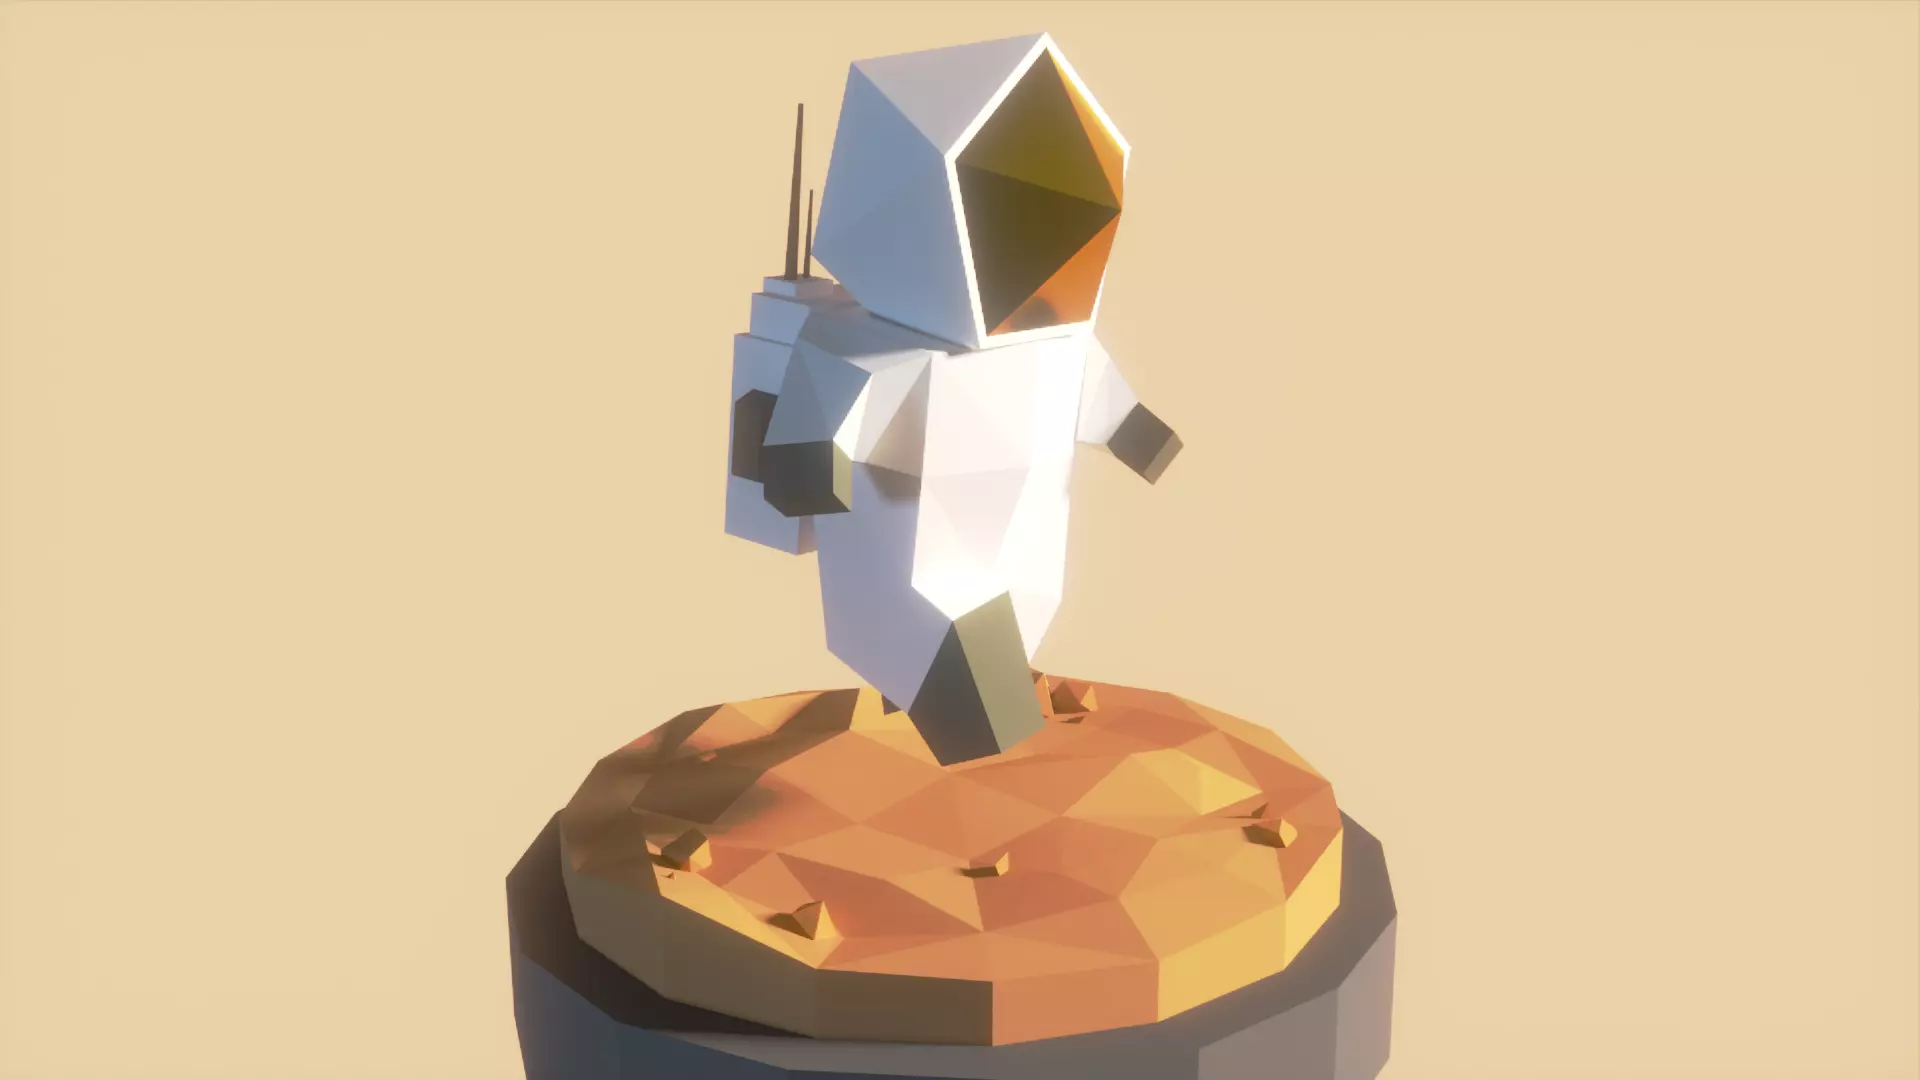
\includegraphics[width=0.9\textwidth, keepaspectratio]{astro}
\caption{Astronaut Asset \cite{astronaut}}
\end{figure}
\end{frame}


\begin{frame}{Thematisierung}
\begin{itemize}
\item Ersetzen der Beans mit dem Astronaut Asset
\end{itemize}
\begin{figure}
    \centering
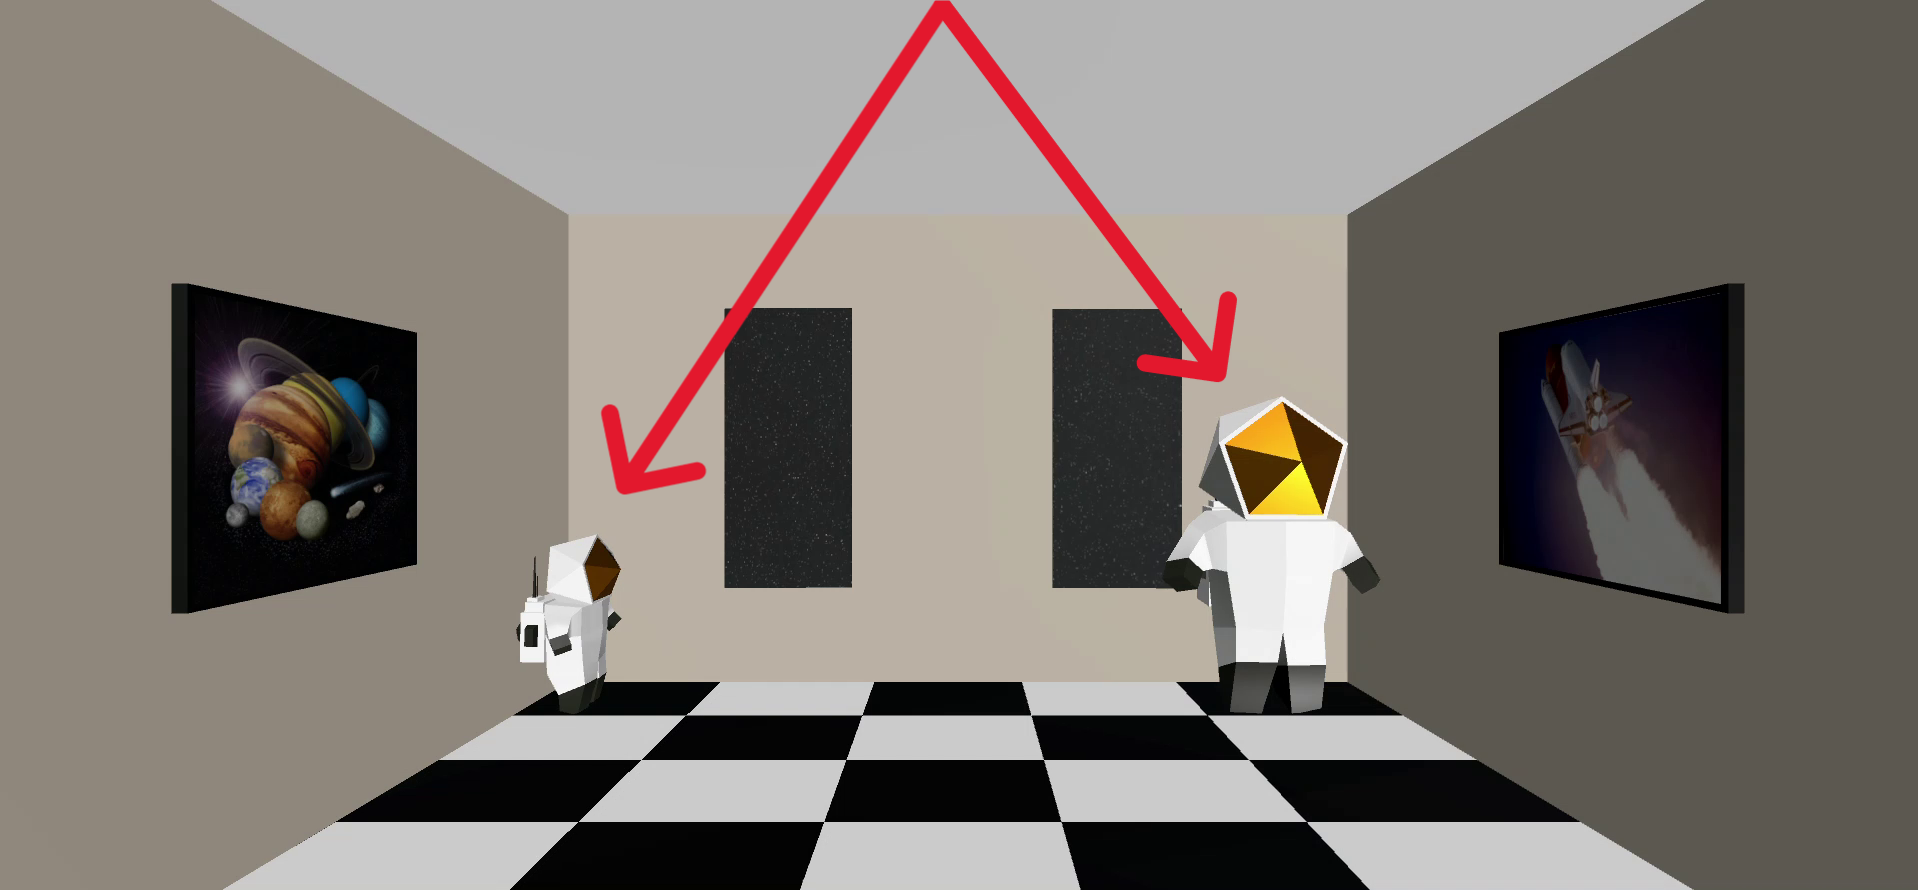
\includegraphics[width=0.9\textwidth, keepaspectratio]{thema1}
\caption{Astronaut Asset \cite{astronaut}}
\end{figure}
\end{frame}


\begin{frame}{Thematisierung}
\begin{itemize}
\item Ersetzen der Prototyp Bilder mit Planeten und Raketen
\end{itemize}
\begin{figure}
    \centering
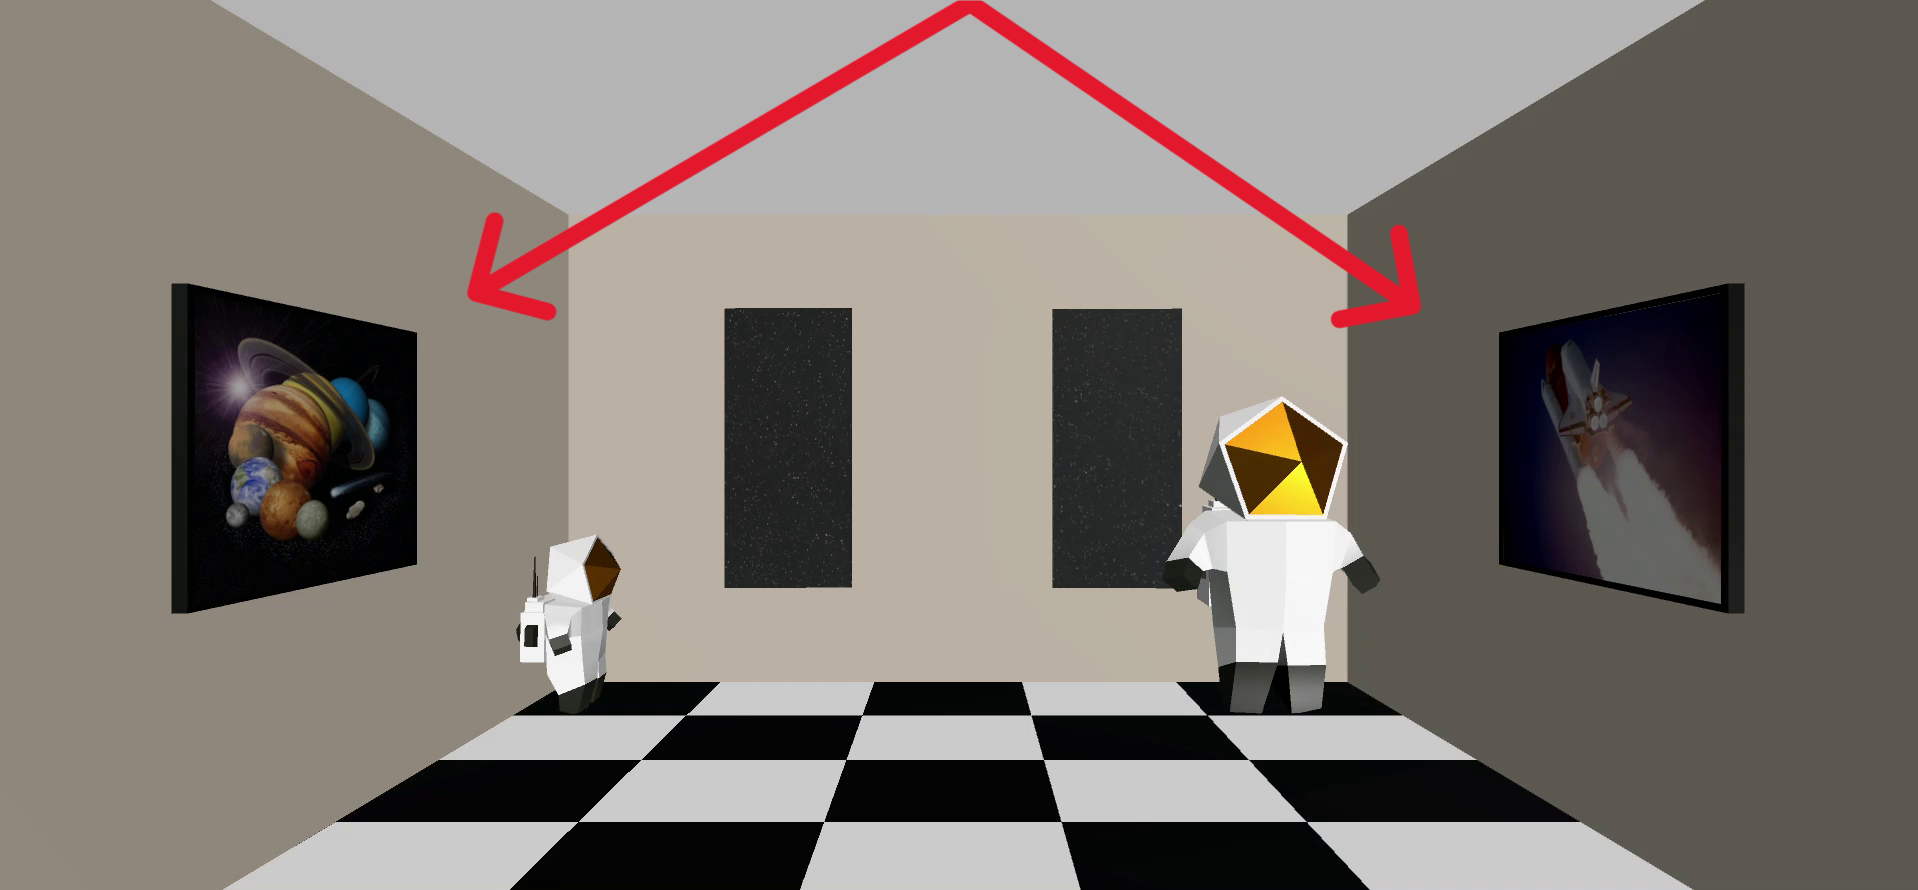
\includegraphics[width=0.9\textwidth, keepaspectratio]{thema2}
\caption{Bilder \cite{rakete} \cite{planet}}
\end{figure}
\end{frame}

\begin{frame}{Thematisierung}
\begin{itemize}
\item Anpassung der Farben an das Thema
\end{itemize}
\begin{figure}
    \centering
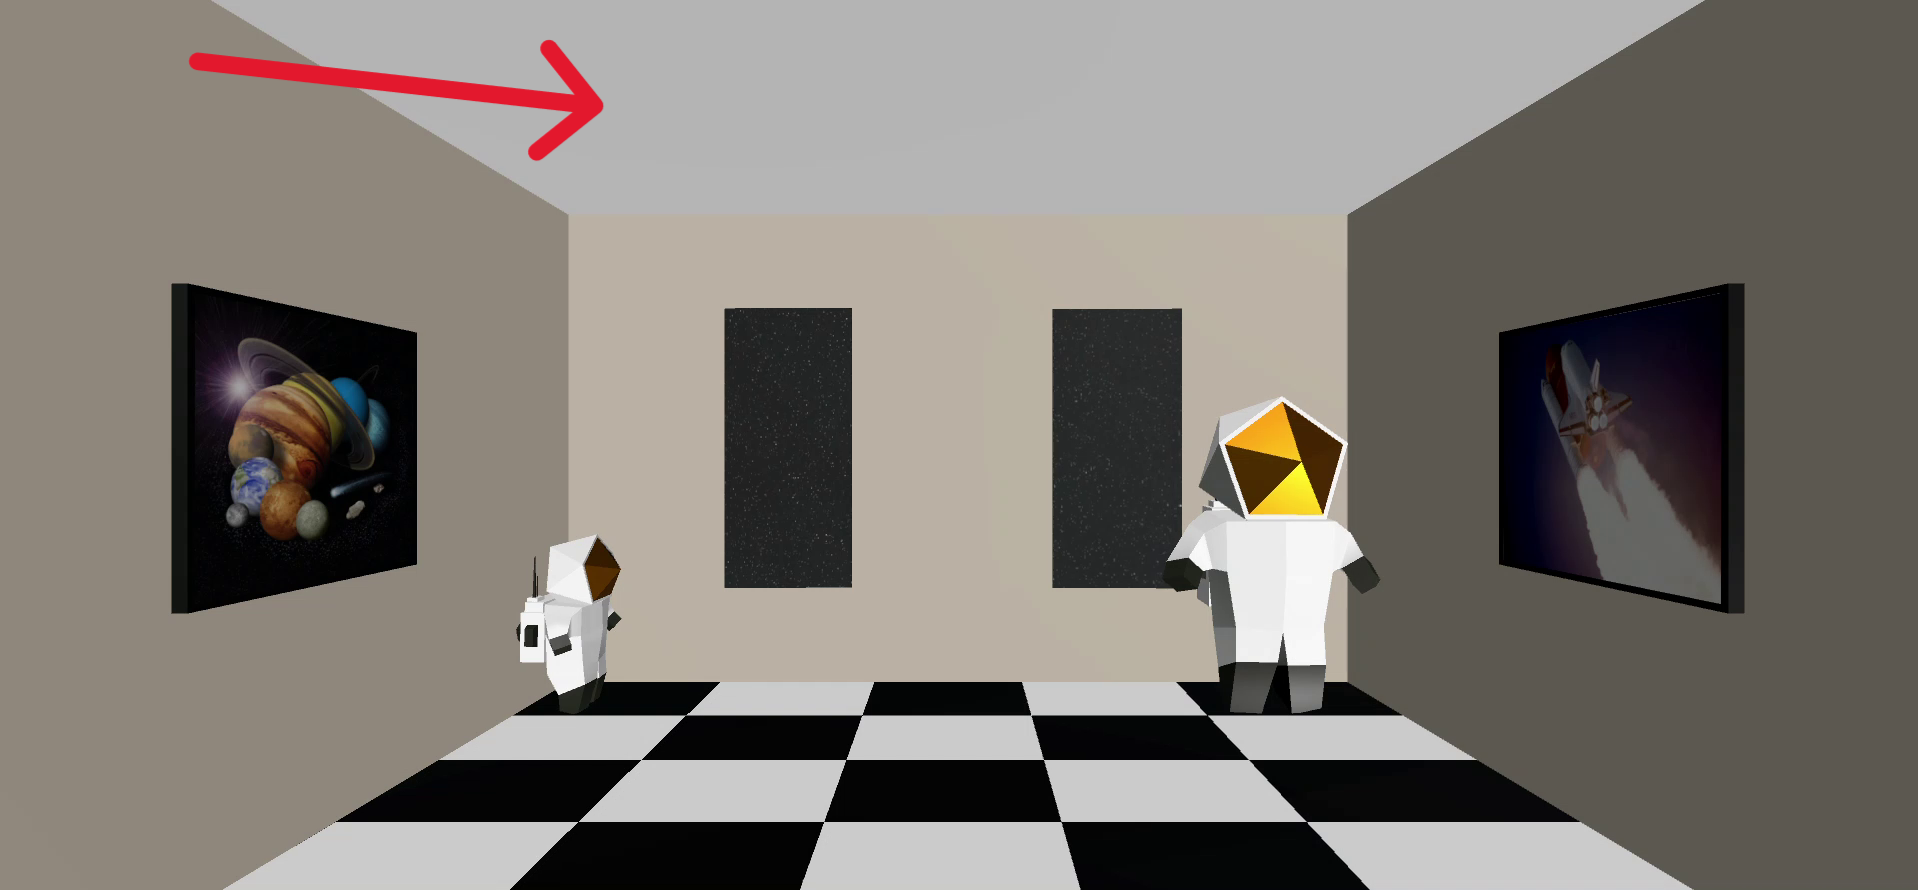
\includegraphics[width=0.9\textwidth, keepaspectratio]{thema3}
\caption{Farbgebung}
\end{figure}
\end{frame}

\begin{frame}{Thematisierung}
\begin{itemize}
\item Hinzufügen eines sich bewegenden Sternenhimmels
\end{itemize}
\begin{figure}
    \centering
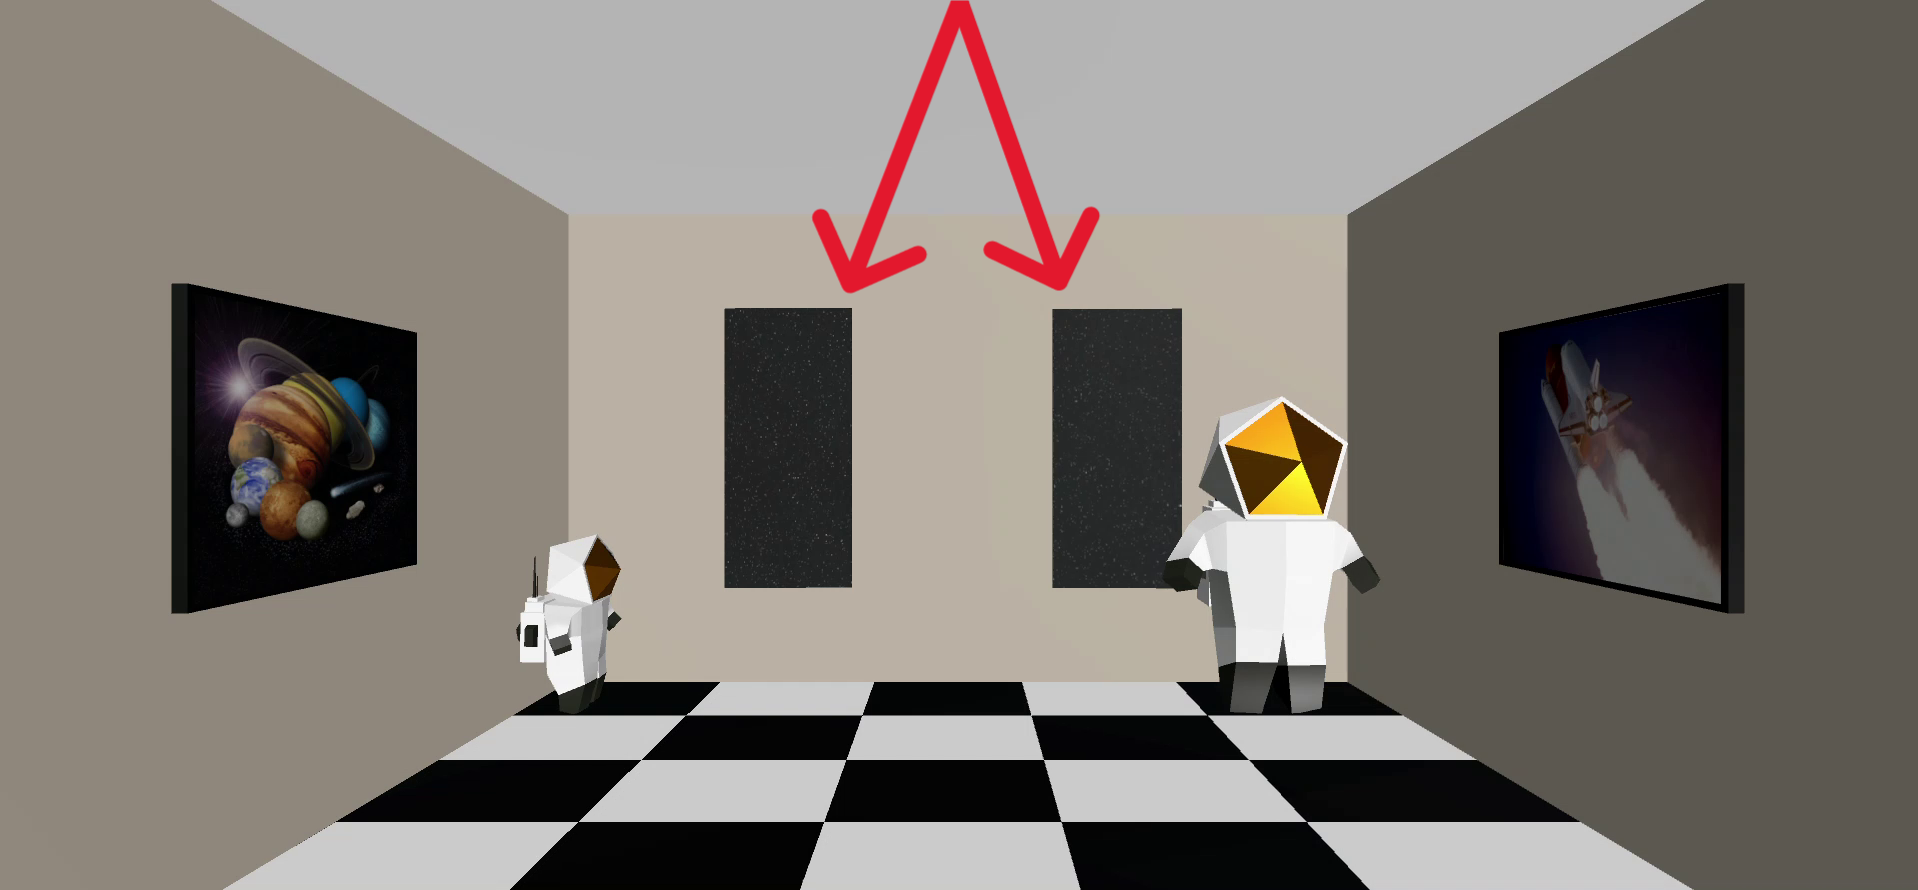
\includegraphics[width=0.9\textwidth, keepaspectratio]{thema4}
\caption{Sternenhimmel \cite{nightsky}}
\end{figure}
\end{frame}

\begin{frame}{Hinzufügen von Skripten}
\begin{itemize}
\item Für die Zwischenwand
\item Für die Astronauten
\item Für die Kamerafahrt
\item Für den Sternenhimmel
\end{itemize}
\end{frame}

\begin{frame}{Aufgabenteil (b)}
\begin{itemize}
\item Illusion in VR erzeugen
\item Illusion durch Bewegung auflösen
\item Illusion durch Werfen von Objekten auflösen
\end{itemize}
\end{frame}


\begin{frame}{VR Illusion}
\begin{figure}
    \centering
    \movie[externalviewer]{
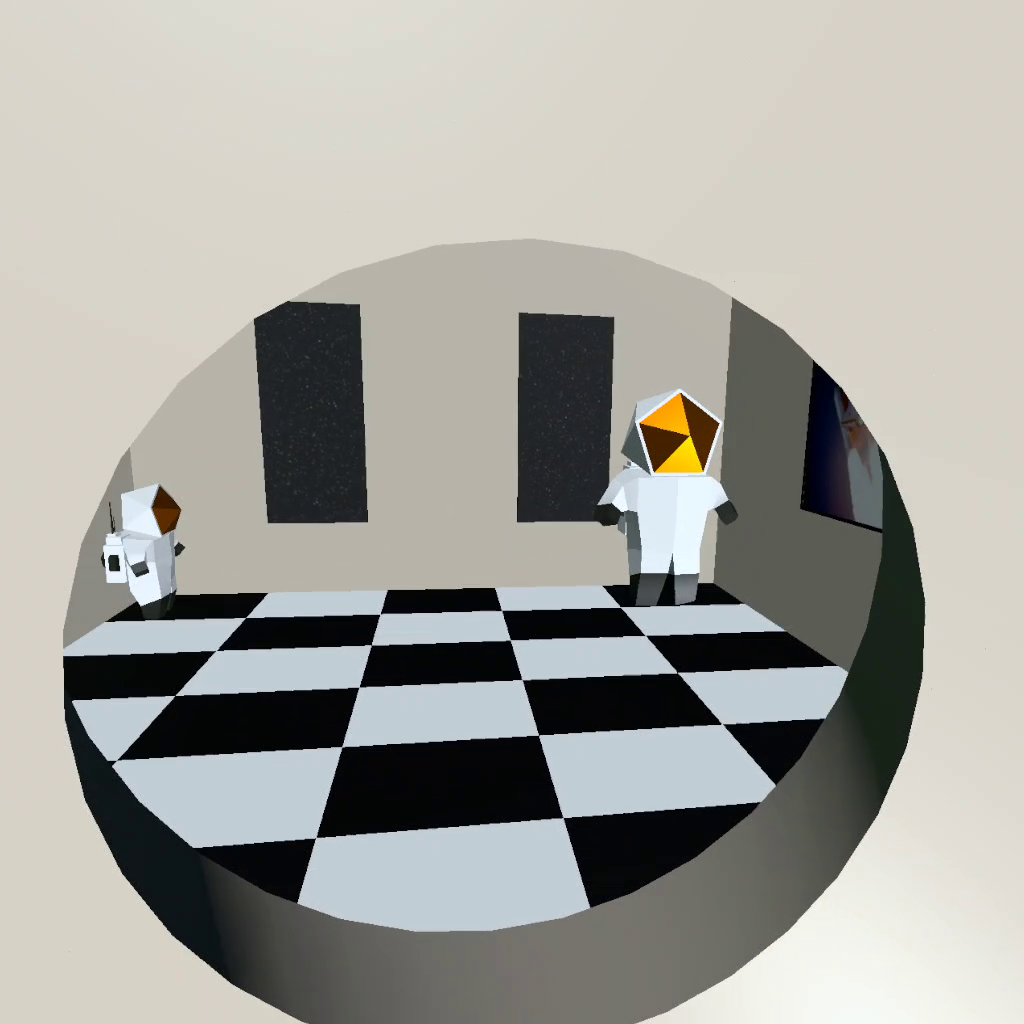
\includegraphics[height=0.8\textheight, keepaspectratio]{VR-Frame}
}{VRMovementAmesRoom.mp4}
\caption{Rundgang in der VR-Umgebung}
\end{figure}
\end{frame}


\begin{frame}{Durchführung}
\begin{itemize}
\item Anpassung der InputActions des XR Interaction Toolkits
\item Anbringen von Mesh Collidern
\item Hinzufügen von unsichtbaren Wänden und Rampe
\item Anfügen des XR Grab Interactable Skripts
\end{itemize}
\end{frame}


\begin{frame}{Quellen}
	\begin{thebibliography}{10}
\bibitem{nick}[1]{ \url{dennisroberts.com/NICKELODEON-AMES-ROOM}
}
\bibitem{astronaut}[2]{ \url{assetstore.unity.com/packages/3d/characters/humanoids/sci-fi/stylized-astronaut-114298}
}
\bibitem{rakete}[3]{ \url{pxhere.com/de/photo/932971}
}
\bibitem{planet}[4]{ \url{pxhere.com/de/photo/1162603}
}
\bibitem{nightsky}[5]{ \url{tools.wwwtyro.net/space-3d/index.html}}
\end{thebibliography}
\end{frame}


	
    	
    	
    	
\end{document}
